\subsection{Durchführung}
Der Aufbau zur Lebensdauermessung ist in Abbildung \ref{fig:lebensdauer_aufbau} zu sehen. Fliegt ein Myon durch den ersten und in den zweiten Szintillationszähler, löst es zwei Signale aus, die zur Koinzidenz führen. Dies ist dann der Startimpuls, der die Zeitmessung startet. Die Zeitmessung geschieht dabei durch das Zählen von Impulsen eines \SI{20}{\mega\hertz}-Oszillators. Damit das Startsignal nicht gleichzeitig auch das Stopsignal ist, wird das Startsignal mit einem Verzögerungskabel um etwa \SI{100}{\nano\second} verzögert. Zerfällt das Myon innerhalb von \SI{10}{\micro\second} in dem zweiten Zähler löst es den Stopimpuls für die Zeitmessung aus. Das Ereigniss wird dann von einem Zählwerk registriert. Das Zählwerk besteht dabei aus zehn Sichtzählern, die jeweils einen Bereich von \SI{1}{\micro\second} abdecken. Kommt nach \SI{10}{\micro\second} kein Stopsignal wird die Zeitmessung zurückgesetzt und kein Ereignis registriert. 

\begin{figure}[h]
  \centering
  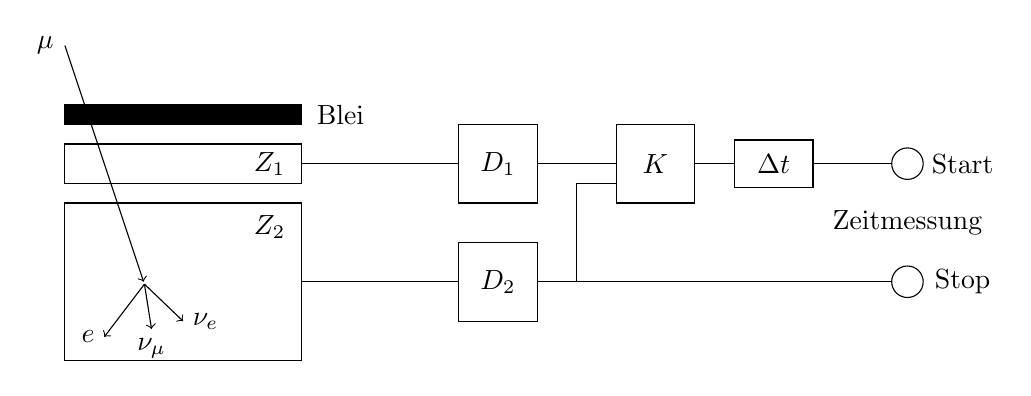
\begin{tikzpicture}
    \draw [fill=black] (0,5) rectangle (3,5.25);
    \draw (3.5,5.125) node {Blei};
    \draw (0,4.25) rectangle (3,4.75);
    \draw (2.6,4.5) node {$Z_1$};
    \draw (0,2) rectangle (3,4);
    \draw (2.6,3.7) node {$Z_2$};
    \draw (3,4.5)--(5,4.5);
    \draw (5,4) rectangle (6,5);
    \draw (5.5,4.5) node {$D_1$};
    \draw (6,4.5)--(7,4.5);
    \draw (7,4) rectangle (8,5);
    \draw (7.5,4.5) node {$K$};
    \draw (8,4.5)--(8.5,4.5);
    \draw (8.5,4.2) rectangle (9.5,4.8);
    \draw (9,4.5) node {$\Delta t$};
    \draw (9.5,4.5)--(10.5,4.5);
    \draw (10.7,4.5) circle (0.2);
    \draw (11.4,4.5) node {Start};
    \draw (3,3)--(5,3);
    \draw (5,2.5) rectangle (6,3.5);
    \draw (5.5,3) node {$D_2$};
    \draw (6,3)--(6.5,3)--(6.5,4.25)--(7,4.25);
    \draw (6.5,3)--(10.5,3);
    \draw (10.7,3) circle (0.2);
    \draw (11.4,3) node {Stop};
    \draw (10.7,3.75) node {Zeitmessung};
    \draw [->] (0,6)--(1,3);
    \draw [->] (1.01,2.97)--(0.5,2.3) node [left] {$e$};
    \draw [->] (1.01,2.97)--(1.5,2.5) node [right] {$\nu_e$};
    \draw [->] (1.01,2.97)--(1.1,2.4) node [below] {$\nu_\mu$};
    \draw (-0.25,6) node {$\mu$};
  \end{tikzpicture}
  \caption{Versuchsaufbau zur Bestimmung der Lebensdauer von Myonen}
  \label{fig:lebensdauer_aufbau}
\end{figure}

Zur Vorbereitung der Messung müssen zunächst die Diskriminatoren und Koinzidenzen eingestellt werden. Dazu werden die Signale $D_1$, $D_2$ und $K$ auf dem Oszilloskop betrachtet. Die Dauer der Ausgangspulse der Diskriminatoren wird nun so eingestellt, dass es zur Überlappung, also zur Koinzidenz kommt (siehe Abbildung \ref{fig:signal_oszi}). Der eingestellte Wert für alle drei Pulse ist $\delta t \approx \SI{25}{\nano\second}$.

\begin{figure}[h]
  \centering
  \begin{tikzpicture}
    \node at (0,0) {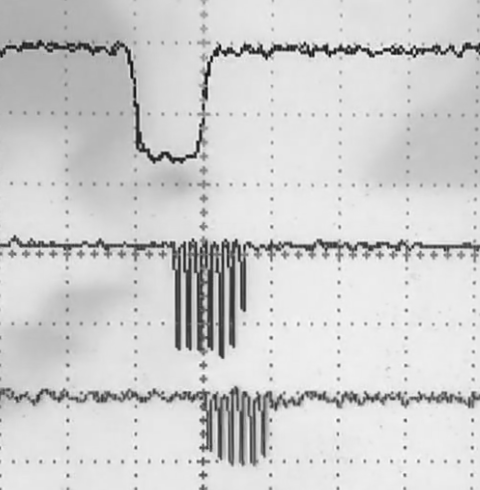
\includegraphics[width=0.5\textwidth]{./data/signal_oszi.png}};
    \draw (-4.5,3.2) node {$D_1$};
    \draw (-4.5,0) node {$D_2$};
    \draw (-4.5,-2.4) node {$K$};
    \draw [<->] (2.6,2) -- (2.6,1);
    \draw (2.1,1.5) node {\SI{0.5}{\volt}};
    \draw [<->] (2.8,1.2) -- (3.8,1.2);
    \draw (3.3,1.5) node {\SI{25}{\nano\second}};
  \end{tikzpicture}
  \caption{Koinzidenz auf Oszilloskop. Oszillationen in Rechteckpulsen von $D_2$ und $K$ werden durch das Oszilloskop verursacht.}
  \label{fig:signal_oszi}
\end{figure}

Zur Einstellung der Schwellenspannungen von $D_1$ und $D_2$ wird jeweils eine Schwellenspannung variiert, während die andere konstant gelassen wird. In einem Monitorkreis werden beide Schwellen auf das Minimum \SI[separate-uncertainty = true]{40.2(1)}{\milli\volt} gestellt. Dieser dient zur Normierung der aus dem ersten Kreis erhaltenen Zählraten. Dann werden die Schwellenspannungen für beide Zähler bestimmt (siehe Auswertung). Die Schwellenspannungen werden eingestellt und die Langzeitmessung mit dem Aufbau aus Abbildung \ref{fig:lebensdauer_aufbau} wird gestartet.
